\chapter{Resultados e Discussão}\label{cap:resultados}

\section{Estrutura do Pedestal}\label{sec:estrutura}
% O protótipo físico será baseado no mecanismo observado na figura \ref{fig:pedestal}. As peças utilizadas no modelo em 3D do pedestal são baseadas em materiais COTS (Commercial off-the-shelf, ou hardware comercial pronto para uso). Então, toda a geometria e os elementos são projetados para serem facilmente encontrados em lojas de materiais de construção.
% As polias utilizadas são GT2 de 20 e 40 dentes, com comprimento de cinto de \SI{10}{\milli\meter}. O cinto utilizado tem \SI{200}{\milli\meter} de comprimento, o que faz com que as distâncias entre centros das polias seja conhecida. Esses elementos são muito utilizados na confecção de impressoras 3D.
% Além das polias, os motores NEMA 17 são costumeiramentes utilizados em impressoas. Os drivers DRV8825 são altamente utilizados para controle de motores de passo, sendo facilmente encontrados em lojas de eletrônicos. O microcontrolador ESP 32 e o display de LCD podem ser encontrados tão facilmente quanto o restante dos componentes eletrônicos.
% O poste no qual o pedestal é dimensionado para utilizar uma viga de madeira de \SI{7,5}{\centi\meter} por \SI{7,5}{\centi\meter}, enquanto as dimensões da base são feitas para utilizar tábuas de \SI{0,9}{\centi\meter} por \SI{9,5}{\centi\meter}. O fio de cobre macisso utilizado para a confecção da antena foi obtido a partir de um cabo para aterramento de 7 fios, no qual cada fio individual possui o padrão \SI{10}{AWG}.
% Enquanto a tela de alumínio para o plano Terra foi obtida de uma tela mosquiteira de alumínio de \SI{1}{\meter\squared}. A chapa de alumínio que compõe o plano Terra é feita a partir de um rufo metálico para telhado. Dessa forma, os materiais são facilmente encontrados em lojas de materiais.

% A estrutura da antena foi confeccionada com o auxílio de uma impressora 3D, feita com PLA (ácido polilático). O resultado pode ser visto na figura \ref{fig:pecas_antena}. A baixa densidade do plástico unida com a densidade de material interna à peça (de 20\%) faz com que toda a estrutura da antena pese \SI{233}{\gram}.
% Unida com aproximadamente \SI{82}{\gram} de cobre para construir a antena, \SI{60}{\gram} da chapa de plano Terra, e \SI{225}{\gram} da tela para fazer o cone, o peso final total da estrutura é de aproximadame \SI{600}{\gram}. Dessa forma, essa antena é ideal para operar com os motores descritos na seção \ref{sec:motor_passo}.
% Esse refinamento da antena faz com que haja uma grande compatibilidade com o restante do sistema.

O protótipo físico será baseado no mecanismo apresentado na Figura~\ref{fig:pedestal}. As peças utilizadas no modelo 3D do pedestal empregam componentes COTS (\textit{Commercial Off-The-Shelf}, ou seja, hardware comercial pronto para uso). Dessa forma, a geometria e os elementos foram projetados para utilizar materiais de fácil acesso no comércio local e em lojas de construção.

As polias utilizadas são do tipo GT2, de 20 e 40 dentes, associadas a uma correia dentada de \SI{10}{\milli\meter} de largura e \SI{200}{\milli\meter} de comprimento perimetral, o que estabelece uma distância entre centros conhecida. Esses elementos, assim como os motores de passo NEMA 17, são amplamente empregados na fabricação de impressoras 3D.

Para o acionamento dos motores, foram adotados os drivers DRV8825, comumente encontrados em lojas de eletrônica. O microcontrolador ESP32 e o display LCD seguem a mesma facilidade de aquisição do restante dos componentes eletrônicos.

A estrutura do poste foi dimensionada para utilizar um pontalete de madeira de \SI{7,5}{\centi\meter} $\times$ \SI{7,5}{\centi\meter}, enquanto a base foi projetada para tábuas de \SI{0,9}{\centi\meter} $\times$ \SI{9,5}{\centi\meter}. O fio de cobre maciço usado para a confecção da antena foi obtido a partir do desmembramento de um cabo de aterramento de 7 vias, no qual cada condutor individual possui bitola \SI{10}{AWG}.

A tela de alumínio empregada no plano de terra foi adaptada de uma tela mosquiteira de alumínio de \SI{1}{\square\meter}. Já a chapa metálica complementar do plano de terra foi produzida a partir de um rufo para telhado.

A estrutura de suporte da antena foi confeccionada via impressão 3D em PLA (ácido polilático), conforme ilustrado na Figura~\ref{fig:pecas_antena}. A baixa densidade do polímero somada ao preenchimento interno (\textit{infill}) de \SI{20}{\percent} resultou em uma massa de \SI{233}{\gram} para a estrutura plástica da antena.

Somando-se aproximadamente \SI{82}{\gram} de cobre para a fiação, \SI{60}{\gram} da chapa e \SI{225}{\gram} da tela de alumínio, a estrutura completa da antena apresenta uma massa total de aproximadamente \SI{600}{\gram}. Essa massa reduzida torna o conjunto adequado para a operação com os motores especificados na Seção~\ref{sec:motor_passo}, garantindo a compatibilidade mecânica do sistema.
\section{Levantamento dos Parâmetros do Filtro $\alpha-\beta-\gamma$}

Conforme apresentado na Seção~\ref{sec:implementacao_filtro}, os parâmetros iniciais do filtro foram obtidos a partir de dados de rastreamento de diversos satélites de órbita baixa (LEO). 
Em seguida, aplicou-se um método computacional de varredura sistemática (\textit{grid search}) para a otimização dos coeficientes, variando-se os parâmetros em incrementos de $0,1$ para $\alpha$ e $\beta$, e de $0,01$ para $\gamma$, respeitando estritamente os limites de estabilidade definidos pelo Critério de Jury (Seção~\ref{sec:estimation}).

O desempenho do filtro para cada combinação de parâmetros foi avaliado ao longo das passagens dos satélites por meio do Erro Quadrático Médio (EQM). A partir desses resultados, geraram-se superfícies tridimensionais correlacionando os coeficientes ao menor erro obtido. 
Essa representação permitiu identificar uma região operacional ótima, na qual o filtro $\alpha-\beta-\gamma$ apresenta convergência satisfatória para a maioria das trajetórias orbitais analisadas.

\begin{figure}[htbp]
    \centering
    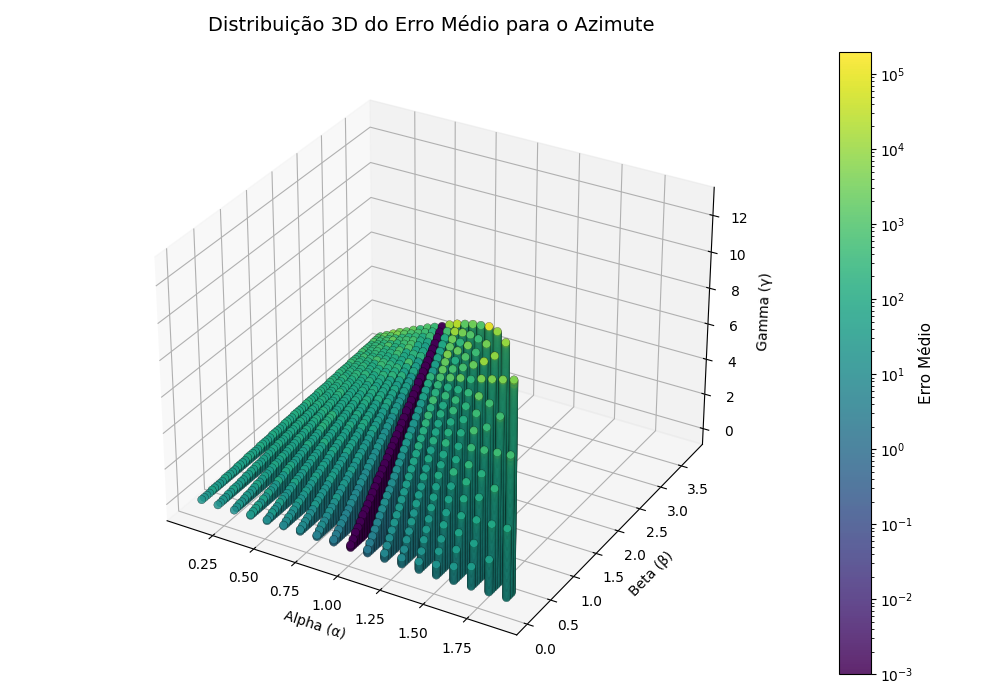
\includegraphics[width=0.8\textwidth]{figs/Plot_alfa_beta_gamma_az.png}
    \caption{Superfície de desempenho dos parâmetros $\alpha$, $\beta$ e $\gamma$ para o eixo de azimute.}
    \caption*{Fonte: Autor (2026)}
    \label{fig:param_az}
\end{figure}

\begin{figure}[htbp]
    \centering
    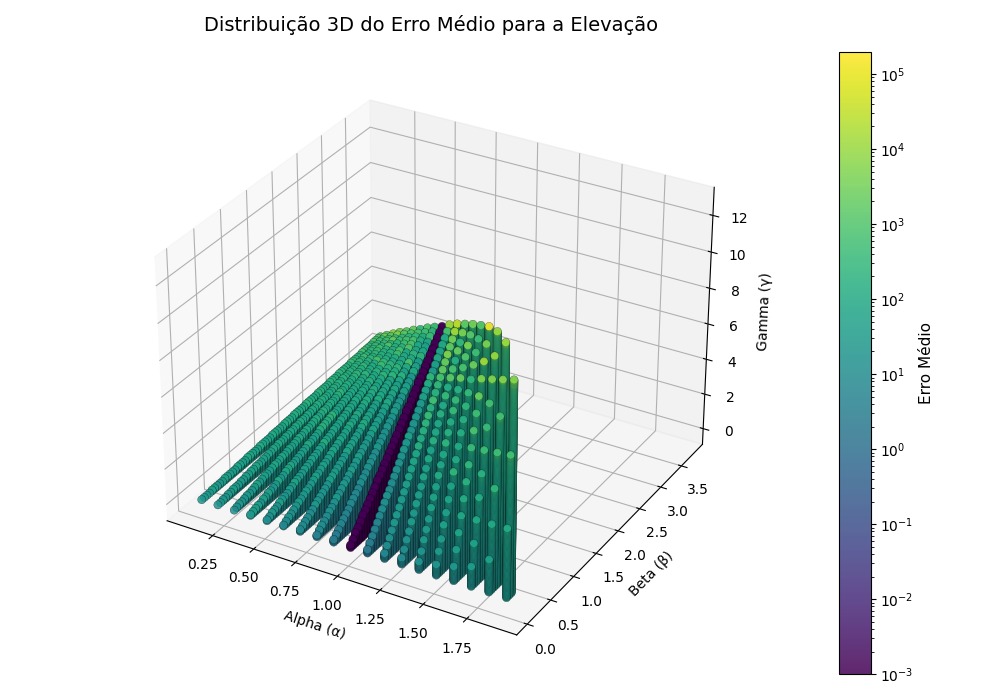
\includegraphics[width=0.8\textwidth]{figs/Plot_alfa_beta_gamma_el.png}
    \caption{Superfície de desempenho dos parâmetros $\alpha$, $\beta$ e $\gamma$ para o eixo de elevação.}
    \caption*{Fonte: Autor (2026)}
    \label{fig:param_el}
\end{figure}

A partir dessa análise, definiram-se os parâmetros do filtro embarcado como $\alpha = 1{,}00$, $\beta = 0{,}05$ e $\gamma = 0{,}00$. Observa-se claramente a existência de uma região onde valores reduzidos de $\beta$ minimizam o erro de estimação. 
Esse comportamento evidencia que a informação orbital fornecida pelo software permite manter a precisão do rastreamento da posição do satélite ao longo da trajetória, sem a introdução de ruídos perceptíveis.

Consequentemente, uma vez estabelecida a estimativa inicial de velocidade do alvo pelo sistema, esta sofrerá apenas variações marginais durante o rastreio. 
Essa característica confere robustez ao pedestal, permitindo que ele continue acompanhando a trajetória do satélite por um período prolongado, mesmo na ocorrência de eventuais interrupções temporárias na comunicação com o software de controle.